\chapter{物理约束温度场世界模型}

温度场世界模型以当前温度场、炉温动作和参数为输入，预测温度增量并递归推演。训练结合参考轨迹误差与离散能量残差。

\section{状态转移表示}

一维模型的离散温度场定义为
\begin{equation}
  \bm{s}_n=[T_1^n,T_2^n,\ldots,T_N^n]^{\mathsf T},\qquad N=41.
\end{equation}
动作 $a_n$ 为区间 $[t_n,t_{n+1})$ 内恒定的炉温设定值，与第\ref{sec:physical-discretization}节一致。参数包含边界参数、导热与比热尺度、密度、厚度和时间步长。密度固定为 \SI{7870}{\kilogram\per\cubic\metre}，保留在序列化输入中。静态工况使用固定参数 $\bm p$，动态边界按步提供 $\bm p_n$。网络预测温度增量
\begin{equation}
  \Delta\widehat{\bm{T}}_n=f_{\theta}(\bm{s}_n,a_n,\bm{p}),\qquad
  \widehat{\bm{s}}_{n+1}=\bm{s}_n+\Delta\widehat{\bm{T}}_n.
  \label{eq:residual_wm}
\end{equation}
式\eqref{eq:residual_wm}定义状态转移 $F_\theta$。递归转移生成给定炉温序列下的轨迹，控制器据此评价候选动作，状态估计器提供当前温度场。

一维主模型采用三隐藏层多层感知机，每层 128 个单元，激活函数为 SiLU。“残差”指预测状态增量，网络内部没有残差块。$h,\varepsilon$ 参数化的输入维数为 $41+1+7=49$，$\Heff$ 参数化为 $41+1+6=48$。输入按训练集统计量标准化，输出温度增量按节点标准化。MLP 接收 41 节点全场，批量评价候选动作。三维实验以卷积网络推进 315 或 1989 个温度状态。

\begin{figure}[H]
  \centering
  \begin{tikzpicture}[
    node distance=9mm and 12mm,
    box/.style={draw=accent,thick,rounded corners=2pt,minimum height=10mm,minimum width=29mm,align=center,fill=accent!5},
    arrow/.style={-{Latex[length=2.2mm]},thick,draw=accent}
  ]
    \node[box] (state) {温度场 $\bm{s}_n$};
    \node[box,below=of state] (action) {炉温动作 $a_n$};
    \node[box,below=of action] (param) {物性与边界参数};
    \node[box,right=18mm of action,minimum width=39mm] (model) {残差世界模型\\$f_\theta$};
    \node[box,right=18mm of model] (next) {预测场 $\widehat{\bm{s}}_{n+1}$};
    \node[box,above=of next] (loss) {数据与物理损失};
    \draw[arrow] (state.east) -- (model.west);
    \draw[arrow] (action.east) -- (model.west);
    \draw[arrow] (param.east) -- (model.west);
    \draw[arrow] (model) -- (next);
    \draw[arrow] (next) -- (loss);
    \draw[arrow] (next.south) |- ++(0,-8mm) -| (state.south);
  \end{tikzpicture}
  \caption{受控递归温度场世界模型}
  \label{fig:architecture}
\end{figure}

\section{递归多步训练与模型选择}

训练样本为长度 $K$ 的连续片段，首步输入参考状态，其余各步输入网络上一时刻的输出，动作序列取自给定工况：
\begin{equation}
  \widehat{\bm{s}}_{n+j+1}=F_{\theta}(\widehat{\bm{s}}_{n+j},a_{n+j},\bm{p}_{n+j}),
  \quad j=0,\ldots,K-1,
\end{equation}
其中 $\widehat{\bm{s}}_n=\bm{s}_n$，一维正式模型取 $K=5$。递归输入包含模型自身的预测偏差。令 $\sigma_{\Delta T,i}$ 为训练集中节点 $i$ 的单步温度增量标准差。多步数据损失为
\begin{equation}
  \mathcal{L}_{\mathrm{data}}
  =\frac{1}{KN}\sum_{j=1}^{K}\sum_{i=1}^{N}
  \left(
    \frac{\widehat{T}_{i}^{n+j}-T_i^{n+j}}{\sigma_{\Delta T,i}}
  \right)^2.
  \label{eq:data_loss}
\end{equation}
梯度由短片段上的多步损失计算，检查点按验证集 300 步完整轨迹 RMSE 选择。归一化统计量取自训练集，测试轨迹不用于选择检查点。

\begin{table}[H]
  \centering
  \caption{一维世界模型的正式训练设置}
  \label{tab:training_config}
  \begin{tabular}{ll@{\hspace{1.8em}}ll}
    \toprule
    项目 & 设置 & 项目 & 设置 \\
    \midrule
    隐藏层 & $3\times128$ & 激活函数 & SiLU \\
    优化器 & AdamW & 初始学习率 & $10^{-3}$ \\
    权重衰减 & $10^{-6}$ & 批量大小 & 512 \\
    训练轮数 & 120 & 展开长度 & $K=5$ \\
    梯度范数上限 & 5 & 随机种子 & 42、7、123 \\
    学习率调度 & 平台期减半 & 最低学习率 & $10^{-5}$ \\
    \bottomrule
  \end{tabular}
\end{table}

\section{离散物理约束}

物理损失采用第\ref{sec:physical-discretization}节与训练数据生成器一致的离散能量平衡。一维内部节点的温度增量残差为
\begin{equation}
  R_i=\widehat{T}_i^{n+1}-T_i^n
  -\frac{\Delta t}{\rho c_{p,i}^{n}\Delta x^2}\left[
  k_{i+1/2}^{n}(\widehat{T}_{i+1}^{n+1}-\widehat{T}_{i}^{n+1})
  +k_{i-1/2}^{n}(\widehat{T}_{i-1}^{n+1}-\widehat{T}_{i}^{n+1})
  \right].
  \label{eq:temperature_residual}
\end{equation}
$R_i$ 的量纲为温度，式中的 $T_i^n$ 表示该次转移的输入状态；多步展开时，后续转移使用网络递归产生的状态。表面节点残差由式\eqref{eq:surface_discrete_balance}左、右两端之差构成，并使用相应的边界换热系数。残差按 $\sigma_{\Delta T,i}$ 归一化，记为 $\widetilde{R}_i=R_i/\sigma_{\Delta T,i}$。多步物理损失写为
\begin{equation}
  \mathcal{L}_{\mathrm{phy}}
  =\frac{1}{K}\sum_{j=1}^{K}
  \frac{1}{N}\sum_{i=1}^{N}\widetilde{R}_{i,n+j}^{2}.
\end{equation}
总损失为
\begin{equation}
  \mathcal{L}=\mathcal{L}_{\mathrm{data}}+\lambda_{\mathrm{phy}}\mathcal{L}_{\mathrm{phy}}.
  \label{eq:total_loss}
\end{equation}
一维单种子预扫描包含 $0$、$10^{-3}$、$10^{-2}$ 和 $10^{-1}$。$10^{-1}$ 的场误差明显增大，三种子比较取 $0$、$10^{-3}$ 和 $10^{-2}$。正式设置 $\lambda_{\mathrm{phy}}=10^{-3}$ 对应最低验证轨迹 RMSE 均值。三维模型采用同类控制体残差，权重与训练预算单独预设。

离散残差刻画预测对指定数值方程的符合程度，与温度误差分别报告。残差降低不必然提高轨迹精度，也不等同于独立的连续能量守恒检验；BDF 参考轨迹上的半隐式残差还包含时间离散差异。

\section{动态边界的可辨识参数化}
\label{sec:boundary-identifiability}

式\eqref{eq:heff_flux}中，温度响应对 $h$ 和 $\varepsilon$ 的约束取决于观测时刻、表面温度和炉温，参数分解并不总是唯一。

\noindent\textbf{命题 1（瞬时边界热流的局部不可辨识性）}
在固定 $T_s$、$\Tinfty$ 且 $h,\varepsilon$ 均未知时，边界热流只依赖标量组合 $\Heff$，映射 $(h,\varepsilon)\mapsto q_s$ 非单射。

由式\eqref{eq:heff_flux}定义
\begin{equation}
  \Heff(t)=h(t)+\varepsilon(t)h_{\mathrm{rad}}(T_s(t),\Tinfty(t)).
  \label{eq:heff}
\end{equation}
在给定 $T_s$ 和 $\Tinfty$ 的当前瞬时状态下，边界热流对两个参数的灵敏度为
\begin{equation}
  \frac{\partial q_s}{\partial(h,\varepsilon)}
  =(\Tinfty-T_s)\begin{bmatrix}1 & h_{\mathrm{rad}}\end{bmatrix}.
  \label{eq:sensitivity}
\end{equation}
当 $\Tinfty\ne T_s$ 时，该行向量的秩为 1，热流只约束一个标量组合。取保持参数可行性的扰动 $\delta\varepsilon$，只要
\begin{equation}
  \delta h=-h_{\mathrm{rad}}\delta\varepsilon,
\end{equation}
就能在当前状态保持相同热流，命题得证。逐时自由变化的 $h(t)$ 和 $\varepsilon(t)$ 因而没有唯一分解。该结论针对已知炉温与单一表面温度下的灰体热流，包括本文一维对称平板两侧温度相同的情形。若多个不同温度的表面共享同一组参数，分别观测其热流可能增加独立约束；该命题不自动推广到任意三维边界。若参数在一段时间内保持常数，变化的 $h_{\mathrm{rad}}$ 可提供额外历史信息。

在给定当前状态和已执行动作时，$\Heff$ 是瞬时边界热流的充分输入；在本文一维对称平板冻结旧状态物性和辐射等效系数的单步离散中，它也是边界参数的充分组合。初始 $\Heff$ 相同的固定 $(h,\varepsilon)$ 组合不保证连续方程或 BDF 的有限时长转移相同：步内表面温度变化会改变 $h_{\mathrm{rad}}$。候选炉温改变时，$h_{\mathrm{rad}}$ 也随之变化，当前 $\Heff$ 不能单独确定新动作下的边界热流。$\Heff$ 因而不构成整个控制问题的充分统计量。

算例的表面温度为 \SI{300}{\degreeCelsius}，当前炉温为 \SI{700}{\degreeCelsius}。

构造五组满足 $\Heff=\SI{121.675}{\watt\per\square\metre\per\kelvin}$ 的 $(h,\varepsilon)$。当前动作下，各组边界热流的数值差为零。将候选炉温改为 \SI{400}{\degreeCelsius}--\SI{950}{\degreeCelsius} 后，辐射基函数随动作改变，参数组合间的最大热流差达到 \SI{12.03}{\kilo\watt\per\square\metre}，若仅按表面半控制体热容将该热流差换算为 \SI{1}{\second} 的显式局部温升增量，其差为 \SI{9.23}{\degreeCelsius}。该数值只度量冻结状态下的边界强迫差异，没有积分内部导热与边界反馈，不能解释为 BDF 求解后真实表面温度相差 \SI{9.23}{\degreeCelsius}。图\ref{fig:counterfactual_identifiability}显示了参数等效方向及其在反事实动作下的分离。

\begin{figure}[H]
  \centering
  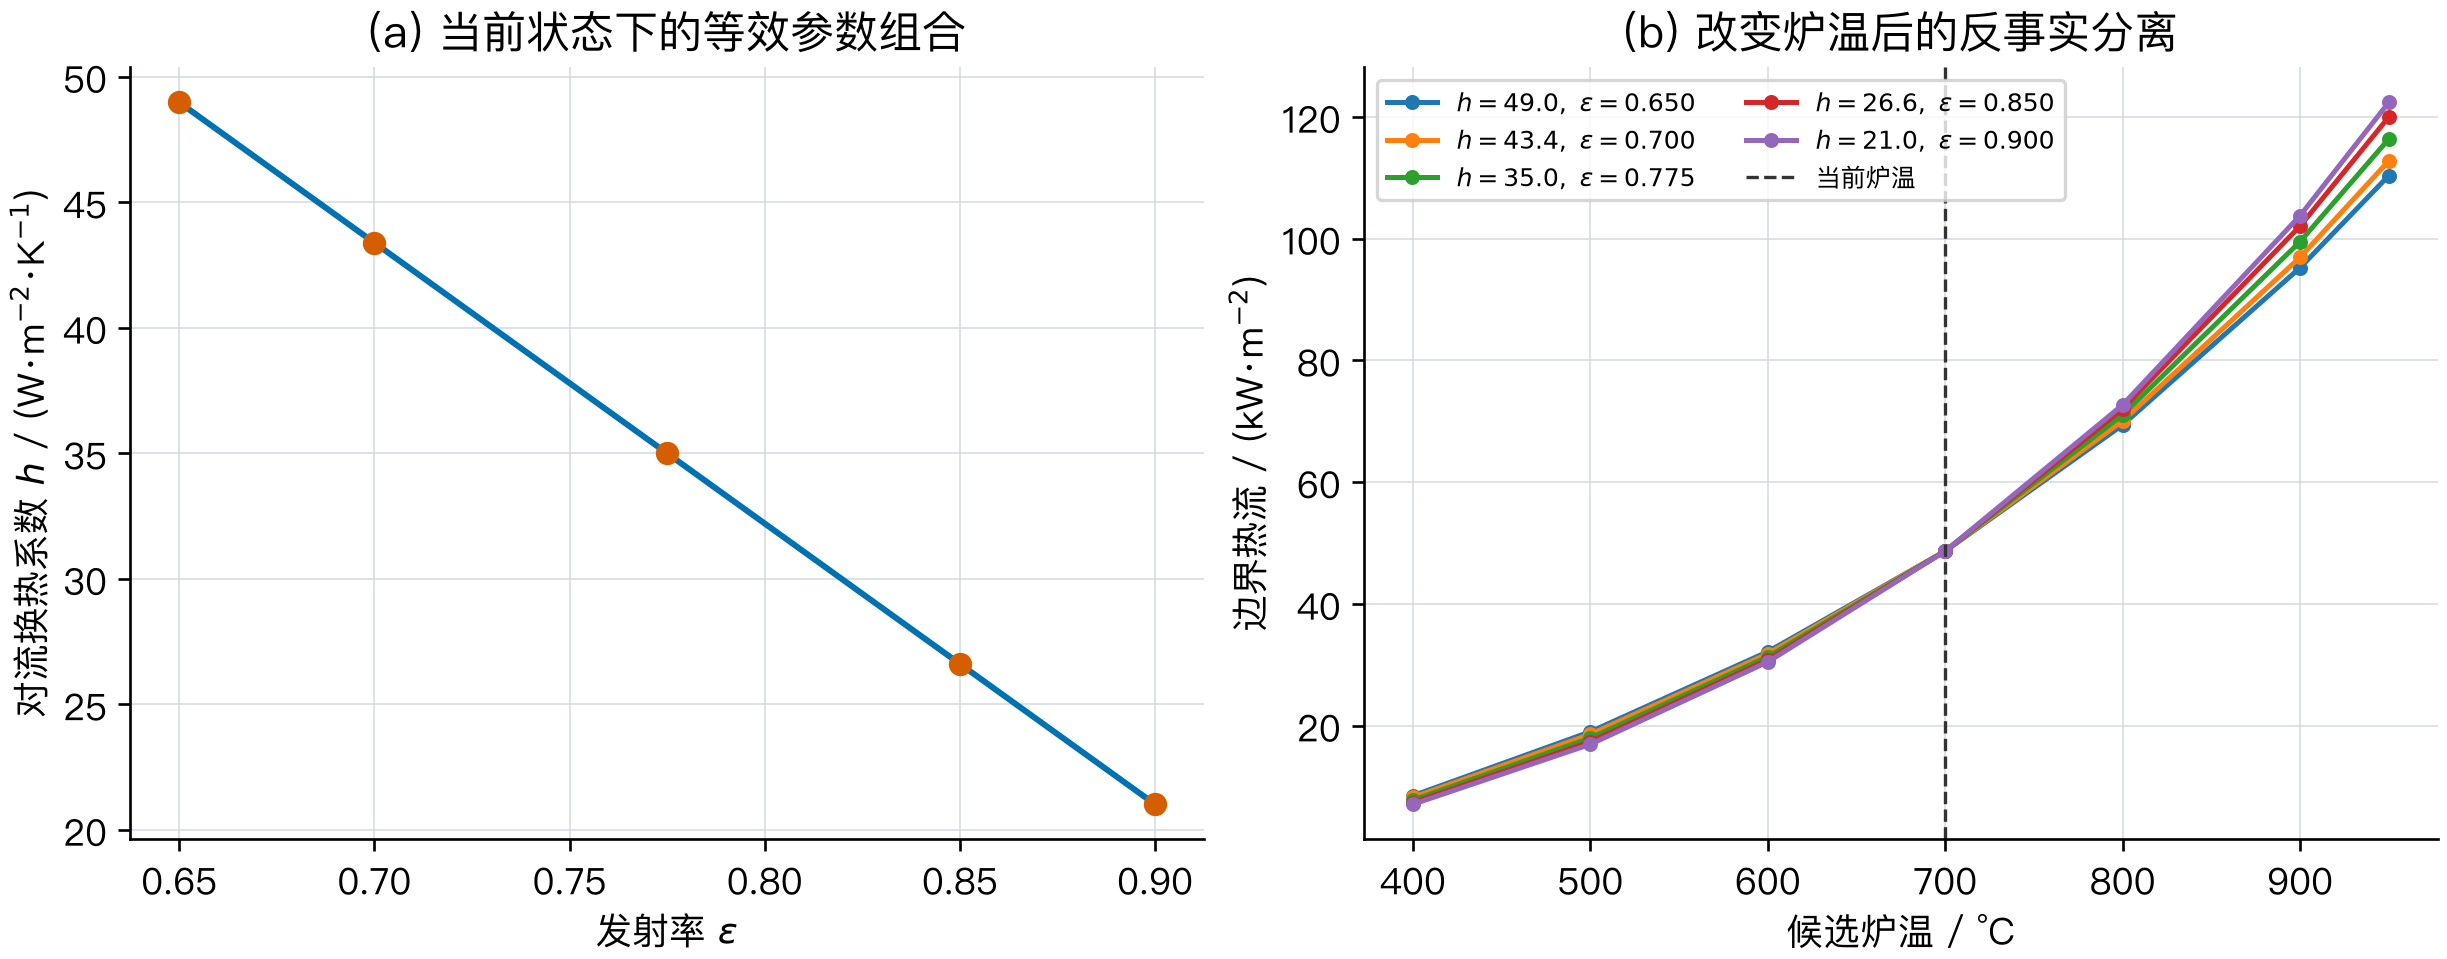
\includegraphics[width=0.98\textwidth]{counterfactual_identifiability.png}
  \caption{当前动作下的等效边界参数与候选炉温改变后的反事实热流}
  \label{fig:counterfactual_identifiability}
\end{figure}

一维等效边界世界模型写为
\begin{equation}
  \widehat{\bm{s}}_{n+1}
  =F_{\theta}^{H}(\bm{s}_n,a_n,\Heff_n,s_k,s_c,L,\Delta t).
  \label{eq:heff_model}
\end{equation}
等效边界表示将当前热流相同的参数组合归为同一输入，降低输入维数。式\eqref{eq:heff_model}省略固定密度，连续参考轨迹上的误差由留出测试评价。

训练和验证中的 $\Heff$ 由参考表面温度构造，接收该序列的完整测试推演属于参考温度条件预测。自主推演给两类模型相同的初态、动作、材料参数与真实动态 $h,\varepsilon$，等效边界模型仅从自身预测表面温度逐步重算 $\Heff$。该比较限于已知外生边界的输入表示，不能直接推定依赖因果观测与状态估计的未知边界应用。

闭环规划通过增广状态滤波器维持受历史测量约束的 $h$ 与 $\varepsilon$ 后验集合，各成员给出候选动作下的 $\Heff(a')$，保留不同参数分解在动作改变后的响应差异。

\section{评价指标与统计单位}
\label{sec:evaluation-protocol}

设测试集包含 $M$ 条轨迹，每条有 $\tau$ 次转移和 $N$ 个温度节点，完整轨迹滚动 RMSE 定义为
\begin{equation}
  \mathrm{RMSE}_{\mathrm{roll}}
  =\sqrt{\frac{1}{MN\tau}\sum_{m=1}^{M}\sum_{n=1}^{\tau}
  \left\|\widehat{\bm{s}}_{m,n}-\bm{s}_{m,n}\right\|_2^2}.
\end{equation}
该指标为全部轨迹、时刻和节点均方误差的平方根。逐轨迹 RMSE 中位数及 95\% 分位数、最大绝对误差、终态 RMSE 和离散物理残差分别描述典型轨迹、尾部、终点误差及方程一致性。最大值原理以当前全场温度与炉温的上下界为全局包络；下一状态越界则记一次违反。该指标允许邻域导热导致的合法升温或降温。

训练重复使用种子 42、7、123。表中“均值$\pm$标准差”默认表示三个训练种子的均值与样本标准差，用于描述训练重复间的变化。每次训练只用验证集选模。一维 BDF 交叉求解器参考及控制环境不用于神经模型训练；三维 BDF 轨迹则按第\ref{sec:dataset-design}节的原则划分后，分别承担训练、验证与测试用途。

方法比较以相同物理工况配对。预测实验的配对差由同一轨迹上两种方法各自的三种子指标均值之差得到，闭环实验按同一 BDF 场景执行相同处理。以轨迹或场景为重采样单位，进行 100000 次配对 bootstrap，报告平均配对差及 95\% 区间。重采样保留同一工况下方法间的对应关系，不把模型种子或轨迹中的时间点计为额外独立工况。逐轨迹 RMSE 的平均配对差与总体滚动 RMSE 的均值之差是不同统计量。

控制成功情况同时报告回合记录与场景判据。对于使用三个训练种子的学习控制器，一个回合对应一个模型在一个场景中的控制过程，场景级成功要求固定的三个模型在该场景均满足成功条件。95\% Wilson 区间以这一场景级二元结果计算，反映固定模型面板在场景抽样下的不确定性。它不等于将三个模型的回合汇总后得到的平均成功率，也不表示任意重训练模型或真实工业炉次的成功保证。温度误差、区间覆盖和控制成功分别评价，单项指标的改善不足以证明闭环整体可靠性。
